\documentclass[11pt,a4paper]{article}

\usepackage[margin=18mm]{geometry}
\usepackage[T1]{fontenc}
\usepackage[utf8]{inputenc}
\usepackage{lmodern}
\usepackage{amsmath}
\usepackage{graphicx}
\usepackage{booktabs}
\usepackage{tabularx}
\usepackage{multirow}
\usepackage{array}
\usepackage{caption}
\usepackage{float}
\usepackage{xcolor}
\usepackage{enumitem}
\usepackage[hidelinks]{hyperref}

\graphicspath{{figures/}}
\captionsetup{font=small,labelfont=bf}
\setlist{nosep,leftmargin=*}
\newcommand{\Id}{I_\mathrm{d}}
\newcommand{\Ig}{I_\mathrm{g}}
\newcommand{\Is}{I_\mathrm{s}}
\newcommand{\Ib}{I_\mathrm{b}}
\newcommand{\Vds}{V_\mathrm{ds}}
\newcommand{\VDD}{V_\mathrm{DD}}

\title{\textbf{ML-Driven PVT-Variation-Aware Leakage Estimation}\\[4pt]
\large Part 2: Transistor-Level ML Models (Training and Model Selection)}
\author{Digital VLSI Design Course Project, 2026\\ Member 2: Pranav Adarsh}
\date{12 November 2026}

\begin{document}
\maketitle

\begin{abstract}
Part 2 replaces SPICE with machine-learning models that predict the four terminal currents
($\Id$, $\Ig$, $\Is$, $\Ib$) of a single 22\,nm transistor from its supply, temperature, geometry,
terminal voltages and process parameters. Four model families (polynomial ridge, random forest,
LightGBM and a multilayer perceptron) were trained and compared for each of the four transistor
cases. The MLP was selected for NMOS ON, NMOS OFF and PMOS OFF, and LightGBM for PMOS ON. Used
inside the gate and circuit models of Parts 3 and 4, the models reach 98.2\% mean accuracy over
3,600 gate simulations and 98.6\% over 102,400 simulations of a 9-input parity checker.
\end{abstract}

\section{Objective and Data}
Each transistor case (NMOS ON, NMOS OFF, PMOS ON, PMOS OFF) has its own SPICE dataset from Part 1,
simulated in ngspice with the 22\,nm MGK model card. Every row holds 12 inputs and 4 targets:
\begin{itemize}
  \item \textbf{Inputs:} $\VDD$ (0.81--0.99\,V), temperature ($-40$ to $125\,^\circ$C), width $W$
        (1--8\,$\times L_\mathrm{min}$), $V_\mathrm{d}$, $V_\mathrm{s}$, $V_\mathrm{g}$, $V_\mathrm{b}$,
        and the process parameters vth0, toxe, ndep, u0 and xj (each $\pm10\%$).
  \item \textbf{Targets:} $\Id$, $\Ig$, $\Is$, $\Ib$ in amperes, positive into the terminal. The
        netlists include drain/source junction areas $AD = AS = W \times 2L_\mathrm{min}$.
\end{itemize}
Each case has 10,000 rows: 5,000 with $V_\mathrm{d}$ and $V_\mathrm{s}$ uniform in $[0,\VDD]$ as the
specification requires, and 5,000 \emph{targeted} rows at the voltages transistors actually see
inside static gates (ON devices at $|\Vds|$ of $\mu$V to mV with one terminal on a rail;
OFF devices with terminals at or near 0 and $\VDD$). Uniform sampling almost never reaches these
points: only 1 of 5,000 uniform PMOS ON rows has $|\Vds| < 4$\,mV with a terminal on $\VDD$,
compared with 2,025 targeted rows.

The uniform and targeted parts are each split 70/15/15 into training, validation and test sets with
a fixed seed (42). Training and validation slices are combined (7,000 and 1,500 rows per case); the
two 750-row test slices are reported separately and used only for the final results.

\section{Method}
\subsection{Target transform and sign model}
Leakage currents span about 15 decades ($10^{-15}$ to $10^{-3}$\,A). A model fitted to raw amperes
would learn only the largest currents, so each current is written as
\begin{equation}
  I = \operatorname{sign}(I)\cdot 10^{y}, \qquad y = \log_{10}|I| .
\end{equation}
A regressor predicts $y$, which makes the training loss proportional to relative error. $\Id$ and
$\Is$ change sign (for $V_\mathrm{d} < V_\mathrm{s}$, or where channel and gate currents cancel), so a
classifier predicts their sign; $\Ig$ and $\Ib$ keep one sign per case, which is stored. All families
share the same LightGBM sign classifier (600 trees): an MLP classifier reached only 94--95\% sign
accuracy near $\Vds \approx 0$, against 99--100\% for LightGBM. Currents below $10^{-15}$\,A (the
SPICE noise floor) are clipped and excluded from the error metrics.

\subsection{Physics-based features}
The 12 raw inputs are extended to about 30 features that expose the device physics: terminal
differences ($\Vds$, $|\Vds|$, $\log_{10}|\Vds|$, $V_\mathrm{gs}$, $V_\mathrm{gd}$, $V_\mathrm{bs}$,
$V_\mathrm{bd}$, and gate/body voltages relative to the lower and higher of $V_\mathrm{d}$,
$V_\mathrm{s}$); $1/kT$ and the logarithms of $W$, toxe, ndep and u0; and subthreshold exponents
such as $(V_\mathrm{gs} - |\mathrm{vth0}|)/kT$ and $\Vds/kT$, which put the exponential leakage
laws on a linear scale. Columns constant within a case are dropped.

\subsection{Metrics}
The relative error $|I_\mathrm{ML} - I_\mathrm{SPICE}| / |I_\mathrm{SPICE}|$ per terminal, summarised
by its median and 95th percentile (p95) as the specification asks, plus $R^2$ on $\log_{10}|I|$.

\section{Models Compared and Selection}
The four families range from a simple, interpretable baseline to a flexible neural network
(Table~\ref{tab:models}).

\begin{table}[H]
\centering
\small
\begin{tabularx}{\linewidth}{>{\raggedright\arraybackslash}p{2.4cm}
                             >{\raggedright\arraybackslash}X
                             >{\raggedright\arraybackslash}X}
\toprule
\textbf{Model} & \textbf{Reason for inclusion} & \textbf{Setup and tuning} \\
\midrule
Polynomial ridge & Baseline; smooth and fast, shows how far a fixed functional form goes &
  Degree 2 or 3 features + ridge ($\alpha = 10^{-3}$ to 1); one multi-output model \\
Random forest & Robust tree ensemble, no scaling needed; standard non-linear reference &
  400 trees, max\_features 0.5 or 1.0; one model per terminal \\
LightGBM & Gradient-boosted trees; usually the strongest model on tabular data &
  Up to 8,000 trees, learning rate 0.03, subsampling 0.8, early stopping (300 rounds) on
  validation; 15--63 leaves; one model per terminal \\
MLP & Smooth function approximator suited to continuous, exponential device physics &
  3 hidden layers $\times$ 64 tanh units, L-BFGS, standardised inputs and outputs; one network
  with 4 outputs \\
\bottomrule
\end{tabularx}
\caption{Model families, rationale and hyperparameter search.}
\label{tab:models}
\end{table}

The MLP is a single network with four outputs, so the terminal currents of a device share what it
learns about the physics; tree models cannot share structure across outputs and get one regressor
per terminal. Full-batch L-BFGS was used instead of Adam because it halved the MLP error in early
tests. Hyperparameters were chosen on the validation set.

\paragraph{Selection rule.} Fixed before any test result was seen: for each case, the family with
the lowest validation score, the mean over the four terminals of $(\text{median} + \text{p95})/2$.
The rule weights accuracy on typical points (median) and on the hardest points (p95) equally.

\section{Results}
\subsection{Model comparison (validation set)}

\begin{table}[H]
\centering
\small
\begin{tabular}{lcccc}
\toprule
\textbf{Case} & \textbf{Poly ridge} & \textbf{Random forest} & \textbf{LightGBM} & \textbf{MLP} \\
\midrule
NMOS ON  & 14.0 / 74 & 13.3 / 68 & 5.8 / 31 & \textbf{2.8 / 29} \\
NMOS OFF & 19.4 / 99 & 9.1 / 51  & 5.5 / 33 & \textbf{2.8 / 12} \\
PMOS ON  & 12.4 / 67 & 12.9 / 61 & \textbf{5.4 / 30} & 2.5 / 37 \\
PMOS OFF & 21.0 / 94 & 9.9 / 52  & 5.5 / 31 & \textbf{2.9 / 13} \\
\bottomrule
\end{tabular}
\caption{Validation median / p95 relative error (\%), mean of four terminals. Bold: model chosen by
the selection rule.}
\label{tab:validation}
\end{table}

\begin{figure}[H]
\centering
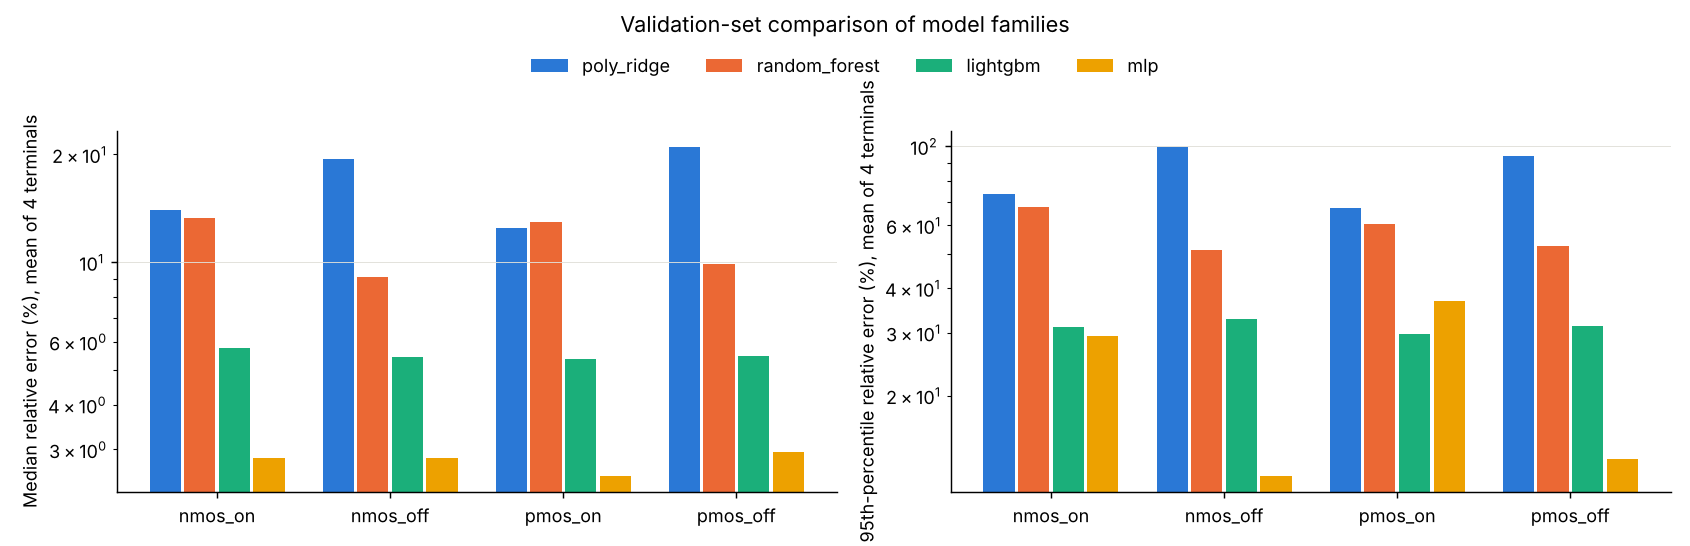
\includegraphics[width=\linewidth]{family_comparison.png}
\caption{Validation error of the four model families per case (log scale): median (left) and p95
(right).}
\label{fig:families}
\end{figure}

The MLP has the lowest median error in every case (2.5--2.9\%), about half of LightGBM's and a fifth
of random forest's (Table~\ref{tab:validation}, Fig.~\ref{fig:families}). Polynomial ridge cannot
follow currents that change by decades across the input range; random forest predicts
piecewise-constant steps (9--13\% median); LightGBM is much better but still steps between leaves,
while the MLP is smooth, like the device equations.

\subsection{Test results of the chosen models}

\begin{table}[H]
\centering
\small
\begin{tabular}{llcccc}
\toprule
\textbf{Case (model)} & \textbf{Test set} & $\boldsymbol{\Id}$ & $\boldsymbol{\Ig}$ &
  $\boldsymbol{\Is}$ & $\boldsymbol{\Ib}$ \\
\midrule
\multirow{2}{*}{NMOS ON (MLP)}      & uniform  & 2.3 / 8  & 1.7 / 7  & 2.3 / 9   & 2.2 / 8  \\
                                    & targeted & 6.6 / 89 & 1.7 / 9  & 7.3 / 100 & 2.3 / 7  \\
\midrule
\multirow{2}{*}{NMOS OFF (MLP)}     & uniform  & 2.1 / 10 & 1.6 / 6  & 2.0 / 11  & 4.9 / 17 \\
                                    & targeted & 2.3 / 10 & 2.1 / 13 & 2.2 / 10  & 7.2 / 26 \\
\midrule
\multirow{2}{*}{PMOS ON (LightGBM)} & uniform  & 3.7 / 21 & 3.9 / 14 & 3.6 / 21  & 8.7 / 27 \\
                                    & targeted & 8.8 / 73 & 2.8 / 13 & 9.2 / 52  & 6.0 / 21 \\
\midrule
\multirow{2}{*}{PMOS OFF (MLP)}     & uniform  & 2.2 / 11 & 1.8 / 7  & 2.1 / 12  & 4.3 / 20 \\
                                    & targeted & 2.4 / 9  & 2.5 / 16 & 2.2 / 9   & 6.2 / 22 \\
\bottomrule
\end{tabular}
\caption{Test-set median / p95 relative error (\%) per terminal, on the held-out uniform and
targeted (gate operating point) sets.}
\label{tab:test}
\end{table}

\begin{figure}[H]
\centering
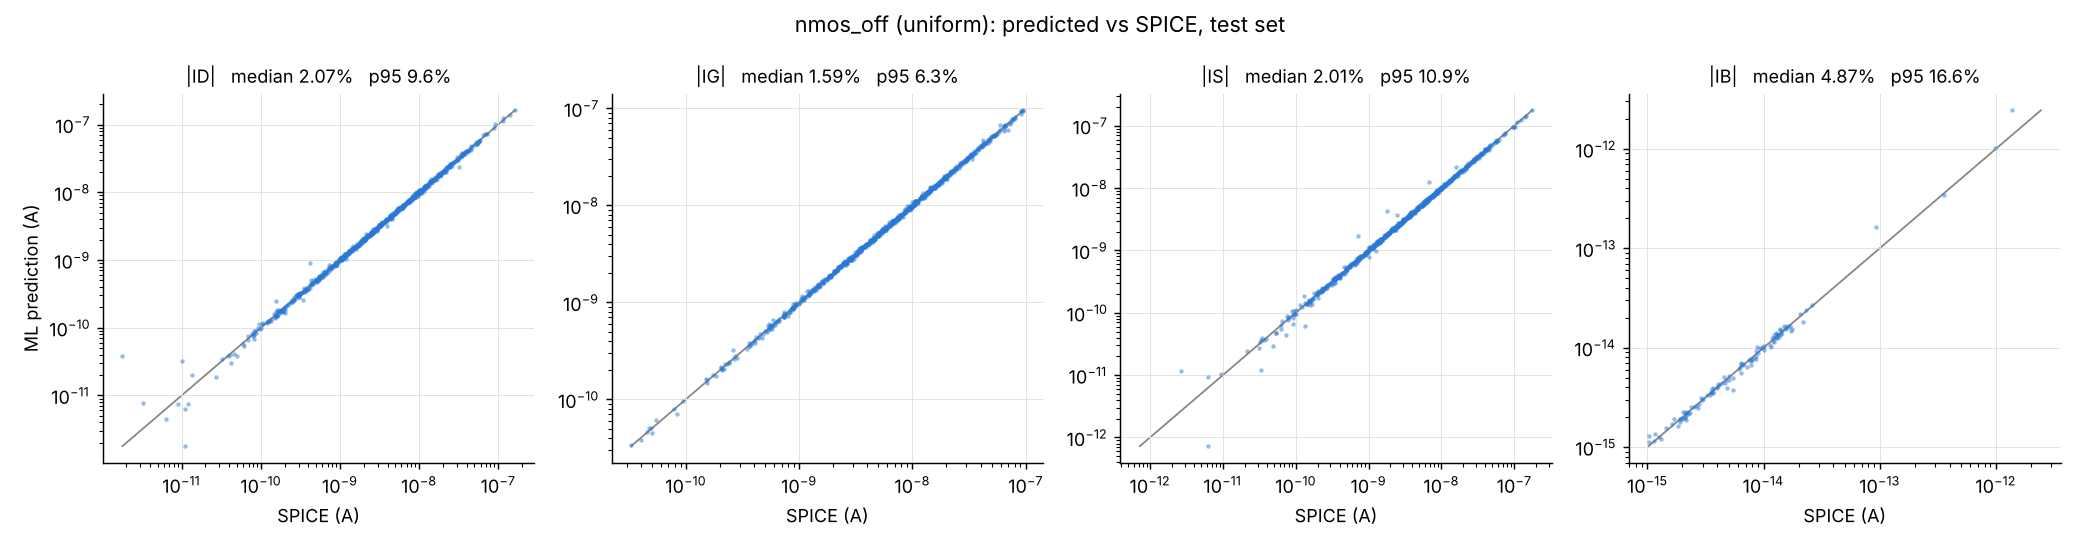
\includegraphics[width=\linewidth]{parity_nmos_off.png}
\caption{Predicted vs SPICE currents on the uniform test set, NMOS OFF (log--log; the line is
$y = x$).}
\label{fig:parity}
\end{figure}

$R^2$ on $\log_{10}|I|$ is at least 0.98 for every terminal and case, and the sign is correct in
98.3--100\% of test rows (Table~\ref{tab:test}, Fig.~\ref{fig:parity}).
\begin{itemize}
  \item \textbf{Typical points:} the MLP cases are at 1.6--2.3\% median error for $\Id$, $\Ig$ and
        $\Is$.
  \item \textbf{Body current of OFF devices} is the hardest regular target (4--7\% median). The
        junction areas roughly double it through junction leakage, a separate mechanism the model
        must learn on top of the channel current.
  \item \textbf{$\Id$ and $\Is$ of ON devices on the targeted set} have large tails (p95 52--100\%).
        At $|\Vds|$ of $\mu$V to mV the channel current passes through zero, so relative
        error divides by almost nothing. The Part 3 gate leakage formula never uses these two
        currents; it uses the ON devices' $\Ig$ and $\Ib$, which are at 1.7--6\% median.
\end{itemize}

\section{Discussion}
\subsection{Choice of LightGBM for PMOS ON}
By the selection rule, LightGBM scores 17.6 and the MLP 19.7 for PMOS ON: the MLP has the better
median (2.5\% vs 5.4\%), but LightGBM the better p95 (30\% vs 37\%), mostly on the hardest
$\Vds \approx 0$ points. The rule's choice was kept so that no model was selected using gate or
circuit test results. Substituting the MLP for PMOS ON was checked only as a variant: gate median
error 1.26\% instead of 1.33\%, circuit mean error 1.33\% instead of 1.40\%, a difference of under
0.1 percentage point.

\subsection{Learning curve}
\begin{figure}[H]
\centering
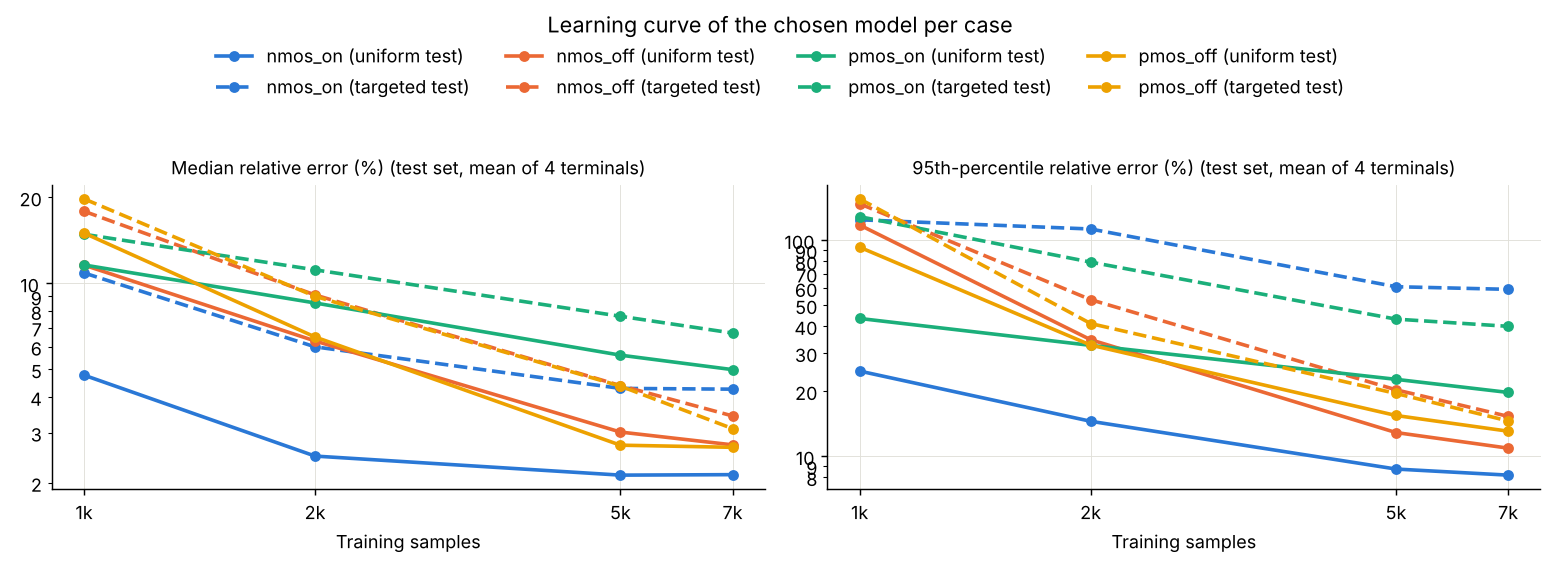
\includegraphics[width=\linewidth]{learning_curve.png}
\caption{Test error of the chosen model per case versus training-set size (solid: uniform test;
dashed: targeted test).}
\label{fig:learning}
\end{figure}

NMOS ON levels off at 5k training rows (2.1\% uniform median). The OFF cases and PMOS ON still
improve from 5k to 7k rows, most on the targeted test (OFF median 4.4\% to 3.1--3.4\%), so more
data, especially targeted OFF rows, would still help (Fig.~\ref{fig:learning}).

\subsection{Accuracy in the gate and circuit models}

\begin{table}[H]
\centering
\small
\begin{tabularx}{\linewidth}{>{\raggedright\arraybackslash}X rccc}
\toprule
\textbf{Level} & \textbf{Runs} & \textbf{Median error} & \textbf{p95 error} &
  \textbf{Mean accuracy} \\
\midrule
Gates: INV, NAND2, NOR2, AND2, OR2 (18 input cases $\times$ 200 corners) & 3,600 & 1.33\% & 4.7\% &
  98.2\% \\
9-input parity checker, corrected estimate (512 vectors $\times$ 200 corners) & 102,400 & 1.14\% &
  3.6\% & 98.6\% \\
\bottomrule
\end{tabularx}
\caption{Accuracy of the Part 2 models when used, without retraining, in Parts 3 and 4.}
\label{tab:downstream}
\end{table}

\begin{figure}[H]
\centering
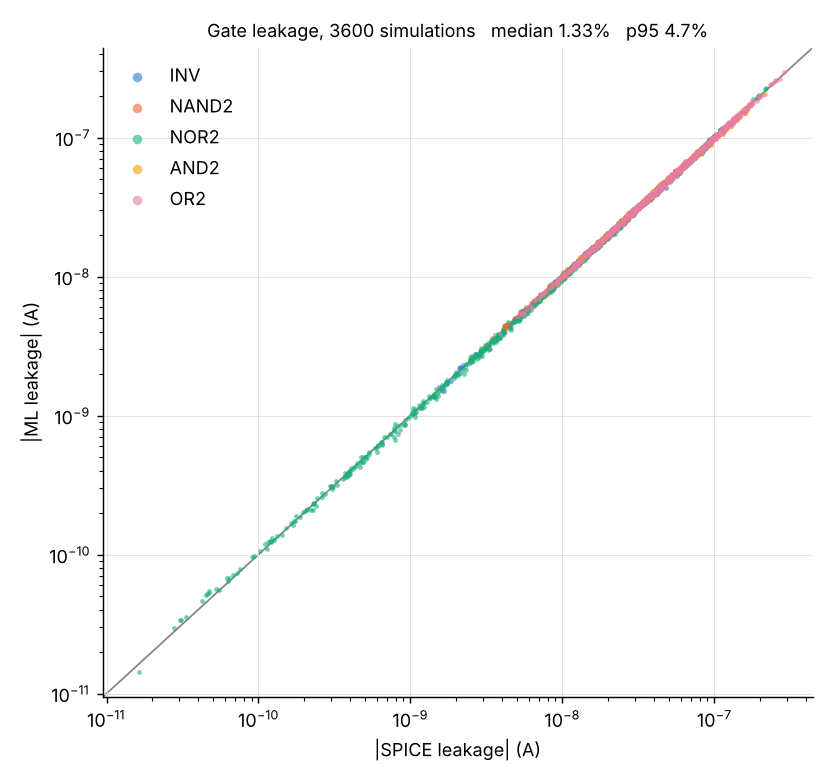
\includegraphics[width=0.55\linewidth]{gate_parity.png}
\caption{Gate leakage, ML vs SPICE, over all 3,600 gate simulations.}
\label{fig:gates}
\end{figure}

Gate and circuit errors are lower than transistor errors (Table~\ref{tab:downstream},
Fig.~\ref{fig:gates}) because leakage there comes from OFF-device and gate currents, which the
models predict well, and errors of separate transistors partly cancel. One gate run in 3,600 has
the wrong sign: NOR2 with inputs 11 at $-38\,^\circ$C, the smallest leakage in the set
($1.6\times10^{-11}$\,A), where two opposite currents nearly cancel.

\subsection{Limitations and next steps}
The 99\% mean-accuracy target is not yet reached (98.6\% at circuit level). The largest remaining
transistor errors are the OFF body current and the ON-device tails at $\Vds \approx 0$. More
targeted training rows, an ensemble of MLPs trained with different seeds, and a larger network are
the most likely improvements.

\section{Reproducibility}
All scripts are in \texttt{part2\_models/} and use fixed seeds:
\begin{itemize}
  \item \texttt{train\_compare.py}: trains and compares all model families and saves the chosen
        models;
  \item \texttt{evaluate\_test.py}: test-set predictions and error tables;
  \item \texttt{learning\_curve.py}: the learning curve.
\end{itemize}
Saved models are in \texttt{results/part2/models/}, one \texttt{.joblib} file per case. The
comparison table, test metrics, hyperparameters, split indices and parity plots are in
\texttt{results/part2/}.

\end{document}
